

{

\addtobeamertemplate{background canvas}{\transfade[duration=0.001]}{}
%gets rid of bottom navigation bars
\setbeamertemplate{footline}[frame number]{}

%gets rid of bottom navigation symbols
\setbeamertemplate{navigation symbols}{}

%gets rid of footer
%will override 'frame number' instruction above
%comment out to revert to previous/default definitions
\setbeamertemplate{footline}{}

\begin{frame}{Fahrplanerstellung in Energiesystemen}
\textbf{Ziel}: Stelle sicher, dass \alert{Erzeugung} (Supply) und \alert{Verbrauch} (Demand) in Balance sind.
\tikzset{
    trajectory/.style={issegrey},
    emph/.style={isseorange},
    trajectorynode/.style={issegrey},
    demand/.style={MidnightBlue, thick},
    firstTraj/.style={ForestGreen},
    secTraj/.style={BrickRed}
} 
\begin{figure}
\begin{tikzpicture}[scale=0.85,transform shape]
    % Draw axes
    \draw [<->,thick] (0,5) node (yaxis) [above] {$P(t)$}
        |- (8.5,0) node (xaxis) [right] {$t$};
        
    \node[overlay,text width=1.9cm, text centered, anchor=south, right] at (7.7,4.5)
    { \small 
    \begin{itemize} 
    \item[] { \color{MidnightBlue} \onslide<2->{\textbf{Demand}} } 
    \item[] { \color{ForestGreen} \onslide<3->{Biogas $a$} } 
    \item[] { \color{BrickRed} \onslide<4->{Biogas $b$} }  
    \item[] { \color{isseorange} \onslide<5->{\textbf{Supply}} }    
    \end{itemize}
    };        
       
	
%	\node[text width = 1.5cm ,text centered, anchor=west, right] at (2.5, 1)
%	{
%		$\mathbf{+}$
%	};
	
    %\node[text width=2.5cm, text centered, anchor=west, right] at (4,-.5)
    %{
    %		Kraftwerk $\mathsf{b}$
	%}; 
	
	%\node[text width = 1.5cm ,text centered, anchor=west, right] at (6.5, 1)
	%{
	%	$\mathbf{=}$
%	};
	%\node[text width=2.5cm, text centered, anchor=west, right] at (8,-.5)
    %{
    %		Demand
	%};      
    
     % draw second trajectory first graph 
     \onslide<2->{
    \draw[trajectory,demand] (0,3.9) coordinate (d20) -- (1,4.6) coordinate (d21);
    \draw[trajectory,demand] (d21) -- (2,4.4) coordinate (d22);
    \draw[trajectory,demand] (d22) -- (3,4.7) coordinate (d23);
    \draw[trajectory,demand] (d23) -- (4,3.5) coordinate (d24);
    \draw[trajectory,demand] (d24) -- (5,3.5) coordinate (d25);
    \draw[trajectory,demand] (d25) -- (6,3.5) coordinate (d26);
    \draw[trajectory,demand] (d26) -- (7,4.0) coordinate (d27);
    \draw[trajectory,demand] (d27) -- (8,4.5) coordinate (d28);
    
    % now for the circles
    \fill[trajectorynode,demand] (d21) circle (1pt);
    \fill[trajectorynode,demand] (d22) circle (1pt);
    \fill[trajectorynode,demand] (d23) circle (1pt);
    \fill[trajectorynode,demand] (d24) circle (1pt);    
    \fill[trajectorynode,demand] (d25) circle (1pt);
    \fill[trajectorynode,demand] (d26) circle (1pt);
    \fill[trajectorynode,demand] (d27) circle (1pt);
    \fill[trajectorynode,demand] (d28) circle (1pt);
    }
        
    \onslide<3->{
    % now for the first plant   
    \draw[trajectory,firstTraj] (0,1.9) coordinate (p10) -- (1,2.0) coordinate (p11);
    \draw[trajectory,firstTraj] (p11) -- (2,2.4) coordinate (p12);
    \draw[trajectory,firstTraj] (p12) -- (3,2.4) coordinate (p13);
    \draw[trajectory,firstTraj] (p13) -- (4,2.2) coordinate (p14);
    \draw[trajectory,firstTraj] (p14) -- (5,2.4) coordinate (p15);
    \draw[trajectory,firstTraj] (p15) -- (6,2.4) coordinate (p16);
    \draw[trajectory,firstTraj] (p16) -- (7,2.4) coordinate (p17);                   
    \draw[trajectory,firstTraj] (p17) -- (8,2.6) coordinate (p18);
    
    	\onslide<6>{
       \draw[trajectory,firstTraj,very thick] (p11) -- (p12);	
       \node[overlay,align=left,rectangle callout,%
             callout absolute pointer=(p11.west),xshift=-.5cm,yshift=-1.5cm,fill=isseorange!50] at (p12) {
            \scriptsize \textbf{Must} ramp up \\ \scriptsize due to inertia};
       
	}    
    
 	\onslide<8>{
       \draw[trajectory,firstTraj,very thick] (p15) -- (p16);	
       \draw[trajectory,firstTraj,very thick] (p16) -- (p17);
       
          \node[overlay,align=left,rectangle callout,%
             callout absolute pointer=(p16.north),xshift=-.5cm,yshift=0.55cm,fill=isseorange!50] at (p15) {
           \scriptsize  Wait 2 steps for \\ \scriptsize further ramp-up};
	} 
	
    % now for the circles of the first graph
    \fill[trajectorynode,firstTraj] (p11) circle (1pt);
    \fill[trajectorynode,firstTraj] (p12) circle (1pt);
    \fill[trajectorynode,firstTraj] (p13) circle (1pt);
    \fill[trajectorynode,firstTraj] (p14) circle (1pt);    
    \fill[trajectorynode,firstTraj] (p15) circle (1pt);
    \fill[trajectorynode,firstTraj] (p16) circle (1pt);
    \fill[trajectorynode,firstTraj] (p17) circle (1pt);
    \fill[trajectorynode,firstTraj] (p18) circle (1pt);        
    }
    
    \onslide<4->{
    % now for the second plant   
    \draw[trajectory,secTraj] (0,2.0) coordinate (p20) -- (1,2.6) coordinate (p21);
    \draw[trajectory,secTraj] (p21) -- (2,2.0) coordinate (p22);
    \draw[trajectory,secTraj] (p22) -- (3,2.2) coordinate (p23);
    \draw[trajectory,secTraj] (p23) -- (4,1.5) coordinate (p24);
    \draw[trajectory,secTraj] (p24) -- (5,1.4) coordinate (p25);
    \draw[trajectory,secTraj] (p25) -- (6,1.2) coordinate (p26);
    \draw[trajectory,secTraj] (p26) -- (7,1.6) coordinate (p27);                   
    \draw[trajectory,secTraj] (p27) -- (8,1.9) coordinate (p28);
	\onslide<6>{
       \draw[trajectory,secTraj,very thick] (p21) -- (p22);	
       \node[overlay,align=left,rectangle callout,%
             callout absolute pointer=(p21.north),xshift=+1cm,yshift=.5cm,fill=isseorange!50] at (p21) {
            \scriptsize Has to compensate};
	}    
	
	\onslide<7>{
       \draw[trajectory,secTraj,very thick] (p23) -- (p24);	
       \node[overlay,align=left,rectangle callout,%
             callout absolute pointer=(p24.south),xshift=+1cm,yshift=-.8cm,fill=isseorange!50] at (p24) {
             \scriptsize Cannot ramp down further \\ \scriptsize due to inertia};
	}    
    
     % now for the circles of the second graph
    \fill[trajectorynode,secTraj] (p21) circle (1pt);
    \fill[trajectorynode,secTraj] (p22) circle (1pt);
    \fill[trajectorynode,secTraj] (p23) circle (1pt);
    \fill[trajectorynode,secTraj] (p24) circle (1pt);    
    \fill[trajectorynode,secTraj] (p25) circle (1pt);
    \fill[trajectorynode,secTraj] (p26) circle (1pt);
    \fill[trajectorynode,secTraj] (p27) circle (1pt);
    \fill[trajectorynode,secTraj] (p28) circle (1pt);
    }
    
    \onslide<5->{
    % draw joint production first graph 
    \draw[trajectory,emph] (0,3.9) coordinate (s20) -- (1,4.6) coordinate (s21);
    \draw[trajectory,emph] (s21) -- (2,4.4) coordinate (s22);
    \draw[trajectory,emph] (s22) -- (3,4.6) coordinate (s23);
    \draw[trajectory,emph] (s23) -- (4,3.7) coordinate (s24);
    \draw[trajectory,emph] (s24) -- (5,3.8) coordinate (s25);
    \draw[trajectory,emph] (s25) -- (6,3.6) coordinate (s26);
    \draw[trajectory,emph] (s26) -- (7,4.0) coordinate (s27);
    \draw[trajectory,emph] (s27) -- (8,4.5) coordinate (s28);
    
	% now for the circles of the sum
    \fill[trajectorynode,emph] (s21) circle (1pt);
    \fill[trajectorynode,emph] (s22) circle (1pt);
    \fill[trajectorynode,emph] (s23) circle (1pt);
    \fill[trajectorynode,emph] (s24) circle (1pt);    
    \fill[trajectorynode,emph] (s25) circle (1pt);
    \fill[trajectorynode,emph] (s26) circle (1pt);
    \fill[trajectorynode,emph] (s27) circle (1pt);
    \fill[trajectorynode,emph] (s28) circle (1pt);
    }
    
	\node[text centered, anchor=north] at (1,0) { 1 }; \draw[thick] (1,0.05) -- (1,-.05);
	\node[text centered, anchor=north] at (2,0) { 2 }; \draw[thick] (2,0.05) -- (2,-.05);
	\node[text centered, anchor=north] at (3,0) { 3 }; \draw[thick] (3,0.05) -- (3,-.05);	
	\node[text centered, anchor=north] at (4,0) { 4 }; \draw[thick] (4,0.05) -- (4,-.05);
	\node[text centered, anchor=north] at (5,0) { 5 }; \draw[thick] (5,0.05) -- (5,-.05);
	\node[text centered, anchor=north] at (6,0) { 6 }; \draw[thick] (6,0.05) -- (6,-.05);
	\node[text centered, anchor=north] at (7,0) { 7 }; \draw[thick] (7,0.05) -- (7,-.05);	
	\node[text centered, anchor=north] at (8,0) { 8 }; \draw[thick] (8,0.05) -- (8,-.05);
	    

\end{tikzpicture}
\end{figure}  
\end{frame}
}



\begin{frame}{Hierarchisches Energiemanagement} \large

\begin{figure}
\centering
\begin{tikzpicture}[->,>=stealth',shorten >=1pt,auto,node distance=1.3cm,
  thick,main node/.style={circle,fill=black!15,draw,font=\sffamily}]

 \node[hierNode, double, label=north:\only<1->{500}] (tl) {a};
 \node[hierNode, double,label=west:\only<4->{\alert<4>{300}}] (i) [xshift=-.2cm, yshift=-.3cm,below left of=tl] {\alert<3-4>{i}}; 
 \node[hierNode, double,label=east:\only<4->{\alert<4>{200}}] (j) [below right of=tl,yshift=-.3cm,xshift=.9cm] {\alert<3-4>{j}};


 \node[hierNode, cStyle, label=south:\only<8->{60}] (c) [below of=i] {\alert<5-7>{c}}; 
 
 \node[hierNode,bStyle, label=south:\only<8->{140}] (b) [left of=c] {\alert<5-7>{b}}; 
 \node[hierNode, dStyle, label=south:\only<8->{100}] (d) [right of=c] {\alert<5-7>{d}}; 
 \node[hierNode, bStyle, label=south:\only<8->{160}] (e) [right of=d] {\alert<5-7>{e}}; 
 \node[hierNode, dStyle, label=south:\only<8->{40}] (f) [right of=e] {\alert<5-7>{f}}; 
  
 
  \path[every node/.style={font=\sffamily\tiny}]
    (tl) edge node [right] {} (i)
   	     edge node [right] {} (j) 
   	(i) edge node [right] {} (b)
   	     edge node [right] {} (c)
   	     edge node [right] {} (d) 
   	(j) edge node [right] {} (e)
   	     edge node [right] {} (f)      ;   	     
  
\onslide<2-4>{ \node[optboundaries, text width=13.5em, text height = 6.4em] (tlOpt) at (.4,-.4) { };}  
 
\onslide<5->{\node[optboundaries, text width=8.7em, text height = 6.8em] (iOpt) at (-1.2,-2.0) {}; }
 
\onslide<5->{\node[optboundaries, text width=6.3em, text height = 6.8em] (jOpt) at (2.2,-2.0) {};}  
 

\onslide<3-4,9->{  
\node[overlay,align=left,rectangle callout,%
      callout absolute pointer=(tl.west),fill=isseorange!50] at (-3.8,-0.3) {Was sollen $i$ und $j$\\ beisteuern?};} 
     
\onslide<4,9->{     
\node[overlay,rectangle callout,%
      callout absolute pointer=(j.north),fill=isseorange!50] at (3.0,1.4) {Wie kann ich $e$ und $f$ repräsentieren?}; } 

\onslide<6->{
\node[overlay,align=left,rectangle callout,%
      callout absolute pointer=(b.west),fill=CornflowerBlue!50] at (-3.8,-4.3) {Wie vermeide ich \\ meinen Speicher \\über 90\% zu füllen?}; } 
      
\onslide<7-> { \node[overlay,align=left,rectangle callout,%
      callout absolute pointer=(f.east),fill=CornflowerBlue!50] at (4.3,-4.4) {Wie beschreibe ich \\ bevorzugte Abläufe?}; }
      
\onslide<10-> { \node[overlay,align=left, fill=issegrey!20] at (0.3,-4.4) {\footnotesize Constraint Relationships / PVS \\
\footnotesize \CustomCite{SGAI'13}, \CustomCite{ICTAI'14} \\
\footnotesize \CustomCite{Wirsing'15}, \alert{\CustomCite{Constraints'17}}
}; }      

\onslide<11-> { \node[overlay,align=left, fill=issegrey!20] at (-3.2,1.4) {\footnotesize Regio-zentrale Fahrpläne\\
\footnotesize \CustomCite{ICAART'14}, \CustomCite{SAOS'14} \\
\footnotesize Marktbasiert \\
\footnotesize \CustomCite{TAAS'15}
}; }      

\onslide<12-> { \node[overlay,align=left, fill=issegrey!20] at (4.7,0.2) {\footnotesize Abstraktion\\
\footnotesize \CustomCite{ICAART'14}, \CustomCite{TCCI'15} \\
\footnotesize \CustomCite{SASO'15}
}; }  

\onslide<13-> { \node[overlay,align=left, fill=issegrey!20] at (5.3,-2.0) {\footnotesize Supply Automata \\
\footnotesize \CustomCite{SEN-MAS'14} \\
\footnotesize \CustomCite{TCCI'15}
}; }  
\end{tikzpicture}

\label{fig:hierarchical-decomposition}
\end{figure}
\end{frame}

\begin{frame}{Selbstorganisierende Ressourcenflusssysteme}
\textbf{Ziel}: Weise Tasks an Roboter zu, sodass ein korrekter \alert{Ressourcenfluss} entsteht
\begin{center}
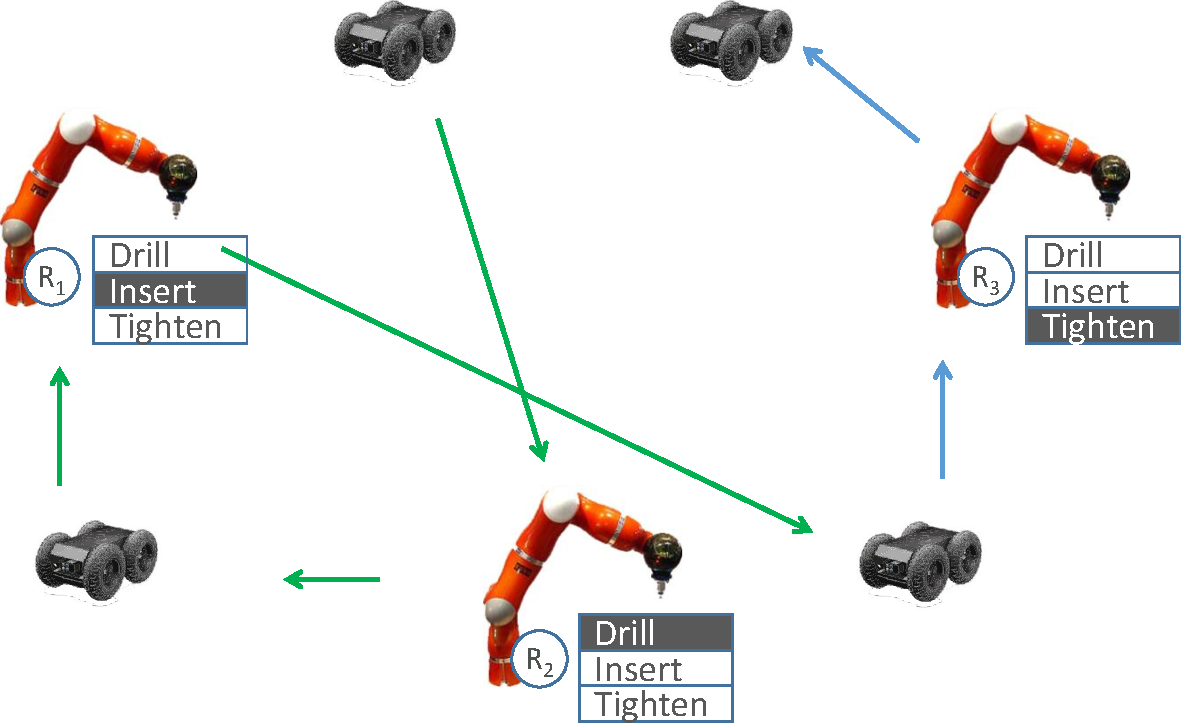
\includegraphics[width=.7\textwidth]{img/produktionszelle.pdf}
\end{center}

\hfill \cite{seebach2010software}

\end{frame}



\begin{frame}[fragile]
\frametitle{Constraint Satisfaction Probleme}

\vspace*{5ex}

\alert{Ziel:} Belege (endlich viele) Variablen aus $X$ mit einem aus (endlich vielen) Werten aus $D$ sodass alle Constraints $C$ erfüllt werden.

\vspace*{1ex}

\textbf{Beispiel}
\begin{itemize}
\item [-] $n$ Roboter, $m$ Tasks
\item [-] Gebe jedem Roboter einen \emph{unterschiedlichen} Task, stelle sicher, dass jeder Task belegt ist 
\end{itemize}

\begin{lstlisting}
% problem data 
int: n; set of int: ROBOTS = 1..n;
int: m; set of int: TASKS = 1..m;

% decisions
array[ROBOTS] of var TASKS: allocation;

% goal
solve satisfy;

% have robots work on different tasks
constraint alldifferent(allocation);
constraint forall(t in TASKS) (exists(r in ROBOTS) (allocation[r] = t));
\end{lstlisting}
\end{frame}

\begin{frame}[fragile]
\frametitle{Constraint Optimization Probleme}

\vspace*{4ex}

\alert{Ziel:} Suche die beste Belegung, sodass eine \textbf{skalare} Zielfunktion $f : [X \to D] \to \mathbb{Z}$ minimiert (oder maximiert) wird.

\vspace*{1ex}

\textbf{Beispiel}
\begin{itemize}
\item [-] $n$ (steuerbare) Supplier, $m$ (steuerbare) Consumer decken Residuallast
\end{itemize}

\begin{lstlisting}
% problem data 
int: n; set of int: SUPPLIERS = 1..n;
array[SUPPLIERS] of int: costs;
int: m; set of int: CONSUMERS = 1..m;
int: residualLoad;

% decisions
array[SUPPLIERS] of var 0..100: supply;
array[CONSUMERS] of var 0..100: demand;

% goal
solve minimize sum(s in SUPPLIERS)(costs[s]*supply[s]);

% have robots work on different tasks
constraint sum(supply) - sum(demand) - residualLoad = 0; 
\end{lstlisting}
\end{frame}

\begin{frame}{Energie: Nicht nur Hard Constraints}

\alert{Harte} Constraints aus Supply Automata:
\begin{equation}
\mathsf{hardBounds}: \forall t \in T, a \in A : m[a][t] = \mathsf{on} \rightarrow P_{\mathrm{min}} \leq S[a][t] \leq P_{\mathrm{max}} \nonumber
\end{equation}

\pause
\vspace*{2ex}
\alert{Weiche} Constraints anlagenspezifisch (z.B. Präferenz für 350 bis 390 KW):
\begin{equation}
\mathsf{ecoSweet}_{\mathsf{bio}}: \forall t \in T : m[\mathsf{biogas}][t] = \mathsf{on} \rightarrow 350 \leq S[\mathsf{biogas}][t] \leq 390 \nonumber
\end{equation}

\pause
\vspace*{2ex}
oder Änderungsgeschwindigkeit
\begin{equation}
\mathsf{inertia}_{\mathsf{therm}}: \forall t \in T : |S[\mathsf{biogas}][t] - S[\mathsf{biogas}][t+1] | \leq 10 \nonumber
\end{equation}
\end{frame}

\begin{frame}
    \frametitle{Soft Constraint Programming in MiniBrass}
 \alert{Constraint Programming}
    \begin{itemize}
    \item Deklarative Programmierung (ähnlich SQL, Prolog)
    \item Trennung von \textbf{Modell} und \emph{Algorithmus}
    \item Geeignet für kombinatorische Probleme unter harten Bedingungen (Physik!)
    \item Modellierungssprache \hFirst{MiniZinc}
    \end{itemize}

    \vspace*{3ex}
    
\alert{Soft Constraint Programming}
    \begin{itemize} 
    \item Modellierung von \textbf{Präferenzen}
    \item Finde Lösungen, die \emph{so gut wie möglich} sind
    \item Was bedeutet ``gut``?
    \item Modellierungssprache \hFirst{MiniBrass}
     \end{itemize}
\end{frame}


\begin{frame}{Warum MiniZinc?}
\begin{parchment}[Rationale]
\centering 
\alert{Eine Sprache -- viele Solver} 
\end{parchment}
\begin{textblock*}{2.cm}[1,1](\textwidth-.5cm,\textheight-1.03cm)


\includegraphics[width=\textwidth]{img/MiniZn_logo.jpg} 

\end{textblock*}
Unterstützte Solver
\begin{itemize}
\item Gecode (CP)
\item JaCoP (CP)
\item Google Optimization Tools (CP)
\item Choco (CP)
\item G12 (CP/LP/MIP)
\end{itemize}

\end{frame}

\tikzset{
   pvsNode/.style={rectangle, 
                   rounded corners,
                   minimum width=8cm,
                   minimum height=5cm,
                   draw,
                   dashed},
   sigNode/.style={rectangle, draw, solid},
   cpLogo/.style={fill=black,circle,minimum width=.5em},
   main node/.style={rectangle,
                     rounded corners,
   					 fill=black!15,
   					 draw,
   					 minimum width=3.5em,
   					 text centered,
                     inner sep=2.5pt,	 
   					 font=\sffamily\footnotesize
   					},
   weightNode/.style={rectangle,
                     rounded corners,
   					 fill=black,
   					 draw,
   					 minimum width=3.5em,
                     inner sep=2.5pt,	 
   					 font=\sffamily\footnotesize
   					}  					
}

\begin{frame}{Welche Arten von Soft Constraints?}

Was machen wir nun mit \alert{$\mathsf{inertia}_{\mathsf{therm}}$} und 
\alert{$\mathsf{ecoSweet}_{\mathsf{bio}}$}?
\begin{description}

\item[\textbf{Max-CSP}] Erfülle so viele Constraints wie möglich \hfill \hSecond{\cite{FreuderW92}} \pause 
\item[\textbf{Weighted CSP}] Minimiere die Summe der verletzten Constraints nach Gewicht \pause \hfill \hSecond{\cite{shapiro1981structural}}
\item[\textbf{Fuzzy CSP}] Erfülle den (minimalen) Erfüllungsgrad (zwischen 0 und 1) über alle Soft Constraints \hfill \hSecond{\cite{ruttkay1994fuzzy}} \pause 
\end{description} \pause 

\vspace*{1ex}

\ldots und natürlich 

\vspace*{1ex}

\begin{description}
\item[\textbf{Constraint Preferences}] (früher \emph{Constraint Relationships}): Definiere partielle Wichtigkeitsordnung über Constraints; erhebe diese zu Mengen von verletzten oder erfüllten Constraints \hfill \hFirst{\cite{Schiendorfer13}}
\end{description}

\vspace*{1ex}
\begin{parchment}[Zentrale Frage]
$\rightarrow$ Was sind die Gemeinsamkeiten? Was müssen wir ``minimal'' tun?
\end{parchment}
\end{frame}

\begin{frame}{Beispiel: Max-CSP}

\begin{figure}[t]
\centering
\begin{tikzpicture}[>=stealth',shorten >=1pt,anchor=north west] 


\begin{scope}
\node[pvsNode,minimum width=4cm,minimum height=3cm] (outer) at (0,0) {};

% the logo

\begin{scope}[node distance=.6cm]

\draw [shading=axis,bottom color=black!10,top color=white,rounded corners] (0,0) -- (0,-1) -- (1.3,-1) -- (1.7,0) -- (0,0);
\draw(0,-1) -- ($ (outer.north east) + (0,-1) $);


% weighted constraints%s logo
\node[cpLogo,scale=0.7,transform shape,] at (0.3,-.45) {};
\node[cpLogo,scale=0.7,transform shape,draw,fill=white] at (0.6,-.1) {};
\node[cpLogo,scale=0.7,transform shape,] at (0.4,-.75) {};
\node[cpLogo,scale=0.7,transform shape,draw] at (0.65,-.4) {};
\node[cpLogo,scale=0.7,transform shape,] at (0.3,-.45) {};
\node[cpLogo,scale=0.7,transform shape,draw,fill=white] at (0.9,-.6) {};

\node[cpLogo,scale=0.7,transform shape,] at (1.0,-.2) {};
\node[cpLogo,scale=0.7,transform shape,draw,fill=white] at (0.9,-.6) {};

\end{scope}

\node[main node,draw,anchor=west] (limitBu) at ($ (outer.center) + (-1,0.1)$)   {\limitBatteryUsage};

\node[main node, anchor=west, style={font=\sffamily\footnotesize}] (earlyBird) at ($(limitBu.west)+(-.9,-.8)$)  {\earlyBird};

\node[main node, anchor=west, style={font=\sffamily\footnotesize}] (prefBatteryLevel) at ($(limitBu.west)+(1.2,-.6)$)  {\prefBatteryLevel};


\end{scope}

\end{tikzpicture}
oder
\begin{tikzpicture}[>=stealth',shorten >=1pt,anchor=north west] 


\begin{scope}
\node[pvsNode,minimum width=4cm,minimum height=3cm] (outer) at (0,0) {};

% the logo

\begin{scope}[node distance=.6cm]

\draw [shading=axis,bottom color=black!10,top color=white,rounded corners] (0,0) -- (0,-1) -- (1.3,-1) -- (1.7,0) -- (0,0);
\draw(0,-1) -- ($ (outer.north east) + (0,-1) $);


% weighted constraints%s logo
\coordinate (beginLogo) at (0.4,0.0);
\node[cpLogo,anchor=south] (upLogo) at ($(beginLogo)+(0.3,-.45)$) {};

\draw [fill=black] ($(beginLogo)+(0,-.7)$) -- ($(beginLogo)+(0.1,-.4)$) -- ($(beginLogo)+(0.5,-.4)$) -- ($(beginLogo)+(0.6,-.7)$) -- ($(beginLogo)+(0,-.7)$);


\end{scope}

\node[weightNode,text=white,anchor=west,text width=1.5cm,text height=.19cm,align=right] (bg) at ($ (outer.center) + (-1,0.1)$)   {\hfill 78};
\node[main node,draw,anchor=west] (limitBu) at ($ (outer.center) + (-1,0.1)$)   {\limitBatteryUsage};

\node[weightNode,text=white,anchor=west,text width=1.75cm,text height=.19cm,align=right] (bg2) at ($(limitBu.west)+(0,-.5)$)   {\hfill 14};
\node[main node, anchor=west, style={font=\sffamily\footnotesize}] (earlyBird) at ($(limitBu.west)+(0,-.5)$)  {\earlyBird};

\node[weightNode,text=white,anchor=west,text width=1.3cm,text height=.19cm,align=right] (bg3) at ($(earlyBird.west)+(0,-.5)$)   {\hfill 3};
\node[main node, anchor=west, style={font=\sffamily\footnotesize}] (prefBatteryLevel) at ($(earlyBird.west)+(0,-.5)$)  {\prefBatteryLevel};


\end{scope}

\end{tikzpicture}

\vspace*{2ex}

oder 

\begin{tikzpicture}[>=stealth',shorten >=1pt,anchor=north west] 


\begin{scope}
\node[pvsNode,minimum width=4cm,minimum height=3cm] (outer) at (0,0) {};

% the logo

\begin{scope}[node distance=.6cm]

\draw [shading=axis,bottom color=black!10,top color=white,rounded corners] (0,0) -- (0,-1) -- (1.3,-1) -- (1.7,0) -- (0,0);
\draw(0,-1) -- ($ (outer.north east) + (0,-1) $);


% constraint relationship logo
\node[cpLogo] (upLogo) at (.55,-.2) {};
\node[cpLogo,below left of=upLogo] (leftLogo) {};
\node[cpLogo,below right of=upLogo] (rightLogo) {};  

\path[->]
  (leftLogo) edge node [right] {} (upLogo)
  (rightLogo) edge node [right] {} (upLogo)
;
\end{scope}

% spd parameter
\begin{scope}[node distance=.7cm,xshift=3cm,scale=.5,transform shape]

% constraint relationship logo
\node[fill,circle,OliveGreen] (upLogo) at ($ (outer.north east) + (-1.3,-0.2) $) {};
\node[fill,circle,BrickRed,below of=upLogo] (centerLogo) {};
\node[fill,circle,gray,left of=centerLogo] (leftLogo) {};
\node[fill,circle,gray,right of=centerLogo] (rightLogo) {};  
\node[below of=centerLogo,yshift=.4em,font=\Large] {$\mathrm{SPD}$};
\path[->]
  (leftLogo) edge node [right] {} (upLogo)
  (centerLogo) edge node [right] {} (upLogo)
  (rightLogo) edge node [right] {} (upLogo)
;

\end{scope}

% EV


\node[main node, anchor=center,style={font=\sffamily\footnotesize}] (8) at ($ (outer.center) + (0,-.8)$)   {\limitBatteryUsage};

\node[main node, style={font=\sffamily\footnotesize},above right of=8] (4)  {\earlyBird};

\node[main node, style={font=\sffamily\footnotesize},above left of=8] (3) {\prefBatteryLevel};

%\node[text width=2cm, anchor=west, left] at (4.3, 0.3) { CR };
%\node[text width=1cm, anchor=east, left] at (5.3, -2.3) { \textsc{SPD} };


\path[every node/.style={font=\sffamily\tiny},->]
  (8) edge node [right] {} (3)
  (8) edge node [right] {} (4)
;

\end{scope}

\end{tikzpicture}
\end{figure}
\end{frame}
\begin{frame}{Algebra zur Hilfe}

Wir benötigen \ldots 

\begin{itemize}
\item Eine Menge $M$ von Erfüllungsgraden, z.B. $[0.0, 1.0]$ oder $\{0, 1, \ldots k\}$ oder $2^{C_s}$. \pause 
\item Eine partielle Ordnung $\leq_M$ über $M$: $m \leq_M n$ drückt aus, dass $m$ \emph{schlechter} als $n$ ist \pause 
\item Eine Kombinationsoperation $\cdot_M$, um zwei Elemente aus $M$ miteinander zu verrechnen  \pause 
\item Ein bestes Element $\varepsilon_M$, um \emph{volle Zufriedenheit} auszudrücken \pause
\end{itemize}
  
  Gemeinsam nennen wir $(M, \cdot_M, \varepsilon_M, \leq_M)$ eine \textbf{partielle Bewertungsstruktur}.
  
  \hfill \emph{\cite{Gadducci2013,SchiendorferPvs2015}}
\end{frame}


%% block styles
\tikzstyle{sensor}=[draw, fill=blue!20, text width=5em, 
    text centered, minimum height=2.5em,drop shadow]    
    
\tikzstyle{alg} = [sensor, text width=5em, fill=isseorange!20, 
    minimum height=13em, rounded corners, drop shadow]
\tikzstyle{constraint}=[draw, circle, fill=issegrey!20, text width=1.2em, 
    text centered, minimum height=1.5em,drop shadow]
\tikzstyle{domainstore} = [alg, text width=5em, fill=isseorange!40, 
    minimum height=4em, rounded corners]
\tikzstyle{goodc} = [ForestGreen, font=\bfseries]
\tikzstyle{badc} = [Red, font=\bfseries]
\tikzstyle{okayc} = [LimeGreen, font=\bfseries]
        
\tikzset{
vecArrow/.style={
  thick
  }
}

\tikzset{
    mynode/.style={rectangle,rounded corners,draw=black, top color=isseorange!5, bottom color=isseorange!30,
                   very thick, inner sep=\myinnersep*1em, minimum size=3em, text centered, outer sep=0, align=center},
    innernode/.style={mynode, text width=3cm,  minimum height=1.5cm,
                      top color=issegrey!20, bottom color=issegrey!60},
    emphnode/.style={innernode, top color=isseorange!30, bottom color=isseorange!70}
}

% Define distances for bordering
\def\blockdist{2.3}
\def\edgedist{2.5}

  \tikzset{
    invisible/.style={opacity=0},
    visible on/.style={alt={#1{}{invisible}}},
    alt/.code args={<#1>#2#3}{%
      \alt<#1>{\pgfkeysalso{#2}}{\pgfkeysalso{#3}} % \pgfkeysalso doesn't change the path
    },
  }
%  
%\begin{frame}{Traditionelles Constraint-Solving}
%\fontsize{8pt}{7.2}\selectfont
%\begin{center}
%\begin{tikzpicture}
%% First row:
% \node (search) [alg]  {Suche \phantom{$x = 5$} };
% \path (search.east)+(4.6,0) node (propag) [alg,text width =12em]  {};
% \node[below right] at (propag.north west) {Constraint Store $C$};
% 
% \path (propag.west)+(0.8,-1.2) node (c1) [constraint] {$c_1$}; 
% \path (propag.west)+(1.1,-0.2) node (c2) [constraint] {$c_2$}; 
% \path (propag.west)+(2.0,0.4) node (c3) [constraint] {$c_3$}; 
% \path (propag.west)+(3.2,0.7) node (c4) [constraint] {$c_4$};
%  
% \path (propag.east)+(-1.2,-1.2) node (domainstore) [domainstore] {Domain Store $(D_x)_{x \in X}$}; 
% 
% \path [draw,vecArrow, ->] ([yshift=-2em]search.north east) -- node [above,visible on=<2->] {$x\gets5$} ([yshift=-2em]propag.north west);
% \path [draw,vecArrow, <-] ([yshift=2em]search.south east) -- node [above,goodc,visible on=<4->] {$\top$} ([yshift=2em]propag.south west);
% 
% \path [draw, vecArrow, <->] (c1.east) -- node [below,visible on=<3->,goodc] {$\top$} (domainstore.west) ;
% \path [draw,vecArrow, <->] (c2.330) -- node [above right,visible on=<3->,goodc] {$\top$} (domainstore.150) ;
% \path [draw,vecArrow, <->] (c3.290) -- node [right,visible on=<3->,goodc] {$\top$} (domainstore.120) ;
% \path [draw,vecArrow, <->] (c4.south) -- node [right,visible on=<3->,goodc] {$\top$} (domainstore.68) ;
%\end{tikzpicture}
%\end{center}
%\onslide<0>{
%\begin{columns}[c] % contents are top vertically aligned
%     \begin{column}[c]{7cm} % each column can also be its own 
%\begin{itemize}
%\item A set of satisfaction degrees $\mathbb{B} = \{ \bot, \top \}$
%\item A combination operation $\wedge$
%\item A neutral element $\top$
%\item A partial order $(\mathbb{B}, \leq_\mathbb{B})$ with $\top <_\mathbb{B} \bot$.
%\end{itemize}
%\end{column}
%     \begin{column}[c]{4.5cm} 
%     \end{column} 
%\end{columns}
%}
%
%\end{frame}
%
%\begin{frame}{Traditionelles Constraint-Solving}
%\fontsize{8pt}{7.2}\selectfont
%\begin{center}
%\begin{tikzpicture}
%% First row:
% \node (search) [alg]  {Suche $x = 5$};
% \path (search.east)+(4.6,0) node (propag) [alg,text width =12em]  {};
% \node[below right] at (propag.north west) {Constraint Store $C$};
% 
% \path (propag.west)+(0.8,-1.2) node (c1) [constraint] {$c_1$}; 
% \path (propag.west)+(1.1,-0.2) node (c2) [constraint] {$c_2$}; 
% \path (propag.west)+(2.0,0.4) node (c3) [constraint] {$c_3$}; 
% \path (propag.west)+(3.2,0.7) node (c4) [constraint] {$c_4$};
%  
% \path (propag.east)+(-1.2,-1.2) node (domainstore) [domainstore] {Domain Store $(D_x)_{x \in X}$}; 
% 
% \path [draw,vecArrow, ->] ([yshift=-2em]search.north east) -- node [above,visible on=<2->] {$y \gets 4$} ([yshift=-2em]propag.north west);
% \path [draw,vecArrow, <-] ([yshift=2em]search.south east) -- node [below,badc,visible on=<4->] {$\bot$} ([yshift=2em]propag.south west);
% 
% \path [draw, vecArrow, <->] (c1.east) -- node [below,visible on=<3->,badc] {$\bot$} (domainstore.west) ;
% \path [draw,vecArrow, <->] (c2.330) -- node [above right,visible on=<3->,goodc] {$\top$} (domainstore.150) ;
% \path [draw,vecArrow, <->] (c3.290) -- node [right,visible on=<3->,goodc] {$\top$} (domainstore.120) ;
% \path [draw,vecArrow, <->] (c4.south) -- node [right,visible on=<3->,goodc] {$\top$} (domainstore.68) ;
%\end{tikzpicture}
%\end{center}
%\onslide<5->{
%\begin{columns}[c] % contents are top vertically aligned
%     \begin{column}[c]{7cm} % each column can also be its own 
%\begin{itemize}
%
%\item Eine Menge von Bewertungen $\mathbb{B} = \{ \bot, \top \}$
%\item Eine Kombination $\wedge$
%\item Ein neutrales Element $\top$
%\item Eine partielle Ordnung $(\mathbb{B}, \leq_\mathbb{B})$ with $\top <_\mathbb{B} \bot$.
%\end{itemize}
%   \end{column} 
%     \begin{column}[c]{4.5cm} 
%     \end{column} 
%\end{columns}
%}
%\end{frame}

\begin{frame}{Soft-Constraint-Solving}
\fontsize{8pt}{7.2}\selectfont
\begin{center}
\begin{tikzpicture}
% First row:
 \node (search) [alg]  {Search $x = 5$};
 \path (search.east)+(4.6,0) node (propag) [alg,text width =12em]  {};
 \node[below right] at (propag.north west) {Constraint Store $C$};
 
 \path (propag.west)+(0.8,-1.2) node (c1) [constraint] {$c_1$}; 
 \path (propag.west)+(1.1,-0.2) node (c2) [constraint] {$c_2$}; 
 \path (propag.west)+(2.0,0.4) node (c3) [constraint] {$c_3$}; 
 \path (propag.west)+(3.2,0.7) node (c4) [constraint] {$c_4$};
  
 \path (propag.east)+(-1.2,-1.2) node (domainstore) [domainstore] {Domain Store $(D_x)_{x \in X}$}; 
 
 \path [draw,vecArrow, ->] ([yshift=-2em]search.north east) -- node [above,visible on=<2->] {$y \gets 4$} ([yshift=-2em]propag.north west);
 \path [draw,vecArrow, <-] ([yshift=2em]search.south east) -- node [below,okayc,visible on=<4->] {$4$} ([yshift=2em]propag.south west);
 
 \path [draw, vecArrow, <->] (c1.east) -- node [below,visible on=<3->,okayc] {$4$} (domainstore.west) ;
 \path [draw,vecArrow, <->] (c2.330) -- node [above right,visible on=<3->,goodc] {$0$} (domainstore.150) ;
 \path [draw,vecArrow, <->] (c3.290) -- node [right,visible on=<3->,goodc] {$0$} (domainstore.120) ;
 \path [draw,vecArrow, <->] (c4.south) -- node [right,visible on=<3->,goodc] {$0$} (domainstore.68) ;
\end{tikzpicture}
\end{center}
\onslide<5->{
\begin{columns}[c] % contents are top vertically aligned
     \begin{column}[c]{7cm} % each column can also be its own environment
    \begin{itemize}
\item Eine Menge von Bewertungen, z.B., $\{ 0, \ldots, k \}$
\item Eine Kombination $+$
\item Ein neutrales Element $0$
\item Eine partielle Ordnung $(\mathbb{N}, \geq)$ mit $0$ als Top 
\end{itemize}
   \end{column} \pause
     \begin{column}[c]{4.5cm} 
        Genannt \cemph{valuation structure}~\cite{Schiex1995valued}, bei totaler Ordnung, ansonsten \cemph{partial valuation structure}~\cite{Gadducci2013}.
        Ähnlich:  \cite{Bistarelli1999}: c-Semiringe 
     \end{column}
\end{columns}
    
}
\end{frame}


\begin{frame}[fragile]{PVS--Idee}
\begin{center}
\begin{tabular}{l|c|c|c|c}
\textbf{Konkrete PVS-Typen} & $M$ & $\cdot_M$ & $\leq_M$ & $\varepsilon_M$ \\ 
\hline 
Weighted CSP (WCSP)& $\mathbb{N}$ & $+$ & $\geq$ & $0$ \\ 
Cost Function Network (CFN)& $\{0,\ldots,k\}$ & $+$/$\max$ & $\geq$ & $0$ \\ 
Fuzzy CSP & $[0,1]$ & $\min$ & $\leq$  & 1 \\ 
Inclusion Max CSP & $2^{C_s}$ & $\cup$ & $\supseteq$  & $\emptyset$ \\ 
Constraint Preferences (CP)\footnote{$C_s$ is the set of soft constraints, $\supseteq_{\mathsf{SPD}}$ is the SPD-ordering on sets.} &$\mathcal{M}^{\mathrm{fin}} (C_s)$ & $\mcup$ & $\supseteq_{\mathsf{SPD}}$ & $\lbag \rbag$ \\ 
\end{tabular} 
\end{center}

\begin{parchment}[Hauptidee]
Implementiere Lösungsverfahren für Constraint-Probleme, die durch Bewertungsstrukturen geordnet sind. Instantiiere für konkrete Probleme.
\end{parchment}
\end{frame}

\begin{frame}{Beispiel: Kombinationen~\cite{SchiendorferPvs2015}}
\begin{tikzpicture}[>=stealth',shorten >=1pt,anchor=north west] 

%% FIRST OVERALL LAYER 

\draw[CornflowerBlue,thick,fill=white] (-0.4,2.95) rectangle (11.7,-5.1);
\node[CornflowerBlue] at (0, 2.9) {$\ltimes \quad \mathtt{lex}$};
\draw[CornflowerBlue,thick] (-0.4,0.8) -- (11.7,0.8);

% the logo

\begin{scope}[yshift=2.45cm]

\node[pvsNode,minimum width=11.5cm,minimum height=1.6cm] (outer) at (0,0) {};


\begin{scope}[node distance=.6cm]

\draw [shading=axis,bottom color=black!10,top color=white,rounded corners] (0,0) -- (0,-1) -- (1.3,-1) -- (1.7,0) -- (0,0);
\draw(0,-1) -- ($ (outer.north east) + (0,-1) $);


% cost function networks logo

\node at (.1,-.3) {\Huge \EUR};
\node at (.6,-0.1) {\Large $\mathbb{Z}$};

\end{scope}

% spd parameter
\begin{scope}[node distance=.7cm,xshift=1.7cm,scale=.5,transform shape]

% cfn logos
\draw[thick,->] ($(outer.east) + (-1.3,1.4)$) -- ($(outer.east) + (-1.3,0.6)$);
\node[font=\Large,anchor=east] at ($(outer.east) + (-0.5,0.3)$) {$\mathrm{Minimize}$};


\node[font=\Huge,anchor=east] at ($(outer.east) + (-2.7,1.1)$) {$\mathrm{\Max}$};
\node[font=\Large,anchor=east] at ($(outer.east) + (-2.7,0.3)$) {$\mathrm{Maximum}$};

\end{scope}

\node[ anchor=center] at  ($ (outer.center) + (0.2,.1)$) {  $\mathtt{avppGoals}$ };
% EV
\begin{scope}[node distance = 3.5cm]

\node[main node, anchor=center,style={font=\sffamily\footnotesize}] (cm) at ($ (outer.center) + (-3.6,-0.5)$)   {$\mathtt{remainingResidualLoad[1]}$};

\node[main node, anchor=west,style={font=\sffamily\footnotesize},right of=cm] (cf)  {$\mathtt{remainingResidualLoad[2]}$};
\node[main node, anchor=west,style={font=\sffamily\footnotesize},right of=cf] (ck)  {$\mathtt{remainingResidualLoad[3]}$};
\end{scope}

%\node[text width=2cm, anchor=west, left] at (4.3, 0.3) { CR };
%\node[text width=1cm, anchor=east, left] at (5.3, -2.3) { \textsc{SPD} };


\end{scope}

\begin{scope}
\node[pvsNode,minimum width=4cm,minimum height=3cm] (outer) at (0,0) {};

% the logo
\draw[isseorange,thick] (-0.2,0.7) rectangle (11.6,-5);
\draw[isseorange,thick,dotted] (4.5,0.7) -- (4.5,-5);
\node[isseorange] at (0, 0.7) {$\times \quad \mathtt{pareto}$};

\begin{scope}[node distance=.6cm]

\draw [shading=axis,bottom color=black!10,top color=white,rounded corners] (0,0) -- (0,-1) -- (1.3,-1) -- (1.7,0) -- (0,0);
\draw(0,-1) -- ($ (outer.north east) + (0,-1) $);


% constraint relationship logo
\node[cpLogo] (upLogo) at (.55,-.2) {};
\node[cpLogo,below left of=upLogo] (leftLogo) {};
\node[cpLogo,below right of=upLogo] (rightLogo) {};  

\path[->]
  (leftLogo) edge node [right] {} (upLogo)
  (rightLogo) edge node [right] {} (upLogo)
;
\end{scope}

% spd parameter
\begin{scope}[node distance=.7cm,xshift=3cm,scale=.5,transform shape]

% constraint relationship logo
\node[fill,circle,OliveGreen] (upLogo) at ($ (outer.north east) + (-1.3,-0.2) $) {};
\node[fill,circle,BrickRed,below of=upLogo] (centerLogo) {};
\node[fill,circle,gray,left of=centerLogo] (leftLogo) {};
\node[fill,circle,gray,right of=centerLogo] (rightLogo) {};  
\node[below of=centerLogo,yshift=.4em,font=\Large] {$\mathrm{SPD}$};
\path[->]
  (leftLogo) edge node [right] {} (upLogo)
  (centerLogo) edge node [right] {} (upLogo)
  (rightLogo) edge node [right] {} (upLogo)
;
\end{scope}

% EV

\node[ anchor=center] at  ($ (outer.center) + (0.2,.7)$) {  $\mathtt{\ev}$ };



\node[main node, anchor=center,style={font=\sffamily\footnotesize}] (8) at ($ (outer.center) + (0,-.8)$)   {\limitBatteryUsage};

\node[main node, style={font=\sffamily\footnotesize},above right of=8] (4)  {\earlyBird};

\node[main node, style={font=\sffamily\footnotesize},above left of=8] (3) {\prefBatteryLevel};

%\node[text width=2cm, anchor=west, left] at (4.3, 0.3) { CR };
%\node[text width=1cm, anchor=east, left] at (5.3, -2.3) { \textsc{SPD} };


\path[every node/.style={font=\sffamily\tiny},->]
  (8) edge node [right] {} (3)
  (8) edge node [right] {} (4)
;

\end{scope}


%% SECOND PVS 
%%%%%%%%%%%%%%%%%%%
% First Layer
\begin{scope}[xshift=5.2cm]
\node[pvsNode,minimum width=6cm,minimum height=1.8cm] (outer) at (0,0) {};

\draw[CornflowerBlue,thick] (-0.2,0.5) rectangle (6.2,-4.9);
\draw[CornflowerBlue,thick] (-0.2,-2) -- (6.2,-2);
\node[CornflowerBlue] at (0, 0.5) {$\ltimes \quad \mathtt{lex}$};
% the logo

\begin{scope}[node distance=.6cm]

\draw [shading=axis,bottom color=black!10,top color=white,rounded corners] (0,0) -- (0,-1) -- (1.3,-1) -- (1.7,0) -- (0,0);
\draw(0,-1) -- ($ (outer.north east) + (0,-1) $);


% cost function networks logo

\node at (.1,-.3) {\Huge \EUR};
\node at (.6,-0.1) {\Large $\mathbb{Z}$};

\end{scope}

% spd parameter
\begin{scope}[node distance=.7cm,xshift=1.7cm,scale=.5,transform shape]

% cfn logos
\draw[thick,<-] ($(outer.east) + (-1.3,1.4)$) -- ($(outer.east) + (-1.3,0.6)$);
\node[font=\Large,anchor=east] at ($(outer.east) + (-0.5,0.3)$) {$\mathrm{Maximize}$};


\node[font=\Huge,anchor=east] at ($(outer.east) + (-2.7,1.1)$) {$\mathrm{\sum}$};
\node[font=\Large,anchor=east] at ($(outer.east) + (-2.7,0.3)$) {$\mathrm{Sum}$};

\end{scope}

\node[ anchor=center] at  ($ (outer.center) + (0.2,.1)$) {  $\mathtt{\biogas1}$ };
% EV
\begin{scope}[node distance = 1.5cm]

\node[main node, anchor=center,style={font=\sffamily\footnotesize}] (cm) at ($ (outer.center) + (-0.6,-0.5)$)   {$\mathtt{costsMaint}$};

\node[main node, style={font=\sffamily\footnotesize},right of=cm] (cf)  {$\mathtt{costsFuel}$};
\end{scope}

%\node[text width=2cm, anchor=west, left] at (4.3, 0.3) { CR };
%\node[text width=1cm, anchor=east, left] at (5.3, -2.3) { \textsc{SPD} };


\end{scope}

%% SECOND LAYER 
\begin{scope}[xshift=5.2cm,yshift=-2.3cm]
\node[pvsNode,minimum width=6cm,minimum height=2.5cm] (outer) at (0,0) {};

% the logo

\begin{scope}[node distance=.6cm]

\draw [shading=axis,bottom color=black!10,top color=white,rounded corners] (0,0) -- (0,-1) -- (1.3,-1) -- (1.7,0) -- (0,0);
\draw(0,-1) -- ($ (outer.north east) + (0,-1) $);


% constraint relationship logo
\node[cpLogo] (upLogo) at (.55,-.2) {};
\node[cpLogo,below left of=upLogo] (leftLogo) {};
\node[cpLogo,below right of=upLogo] (rightLogo) {};  

\path[->]
  (leftLogo) edge node [right] {} (upLogo)
  (rightLogo) edge node [right] {} (upLogo)
;
\end{scope}

% spd parameter
\begin{scope}[node distance=.7cm,xshift=3cm,scale=.5,transform shape]

% constraint relationship logo
\node[fill,circle,OliveGreen] (upLogo) at ($ (outer.north east) + (-1.3,-0.2) $) {};
\node[fill,circle,BrickRed,below of=upLogo] (centerLogo) {};
\node[fill,circle,BrickRed,left of=centerLogo] (leftLogo) {};
\node[fill,circle,BrickRed,right of=centerLogo] (rightLogo) {};  
\node[below of=centerLogo,yshift=.4em,font=\Large] {$\mathrm{TPD}$};
\path[->]
  (leftLogo) edge node [right] {} (upLogo)
  (centerLogo) edge node [right] {} (upLogo)
  (rightLogo) edge node [right] {} (upLogo)
;

\end{scope}

% BIOGAS Plant 
\begin{scope}[node distance =1.2cm]
\node[main node, anchor=center, style={font=\sffamily\footnotesize}] (gf) at ($ (outer.center) + (0,0)$) {\gasFull};
\node[main node, style={font=\sffamily\footnotesize}] (ecs) [below left of=gf,xshift=5.4] {\ecoSweet};
\node[main node, style={font=\sffamily\footnotesize}] (ono) [below right of=gf,xshift=-3.1] {\onOff};
\end{scope}
%\node[main node, style={font=\sffamily\footnotesize},double] (hardConstraint) [below left of=7,xshift=-3.1,yshift=7] {$\mathsf{maxProd}$};
\node[ anchor=center] at  ($ (outer.center) + (0.2,.7)$) {  $\mathtt{\biogas2}$ };


%\node[text width=2cm, anchor=west, left] at (4.3, 0.3) { CR };
%\node[text width=1cm, anchor=east, left] at (5.3, -2.3) { \textsc{SPD} };


\path[every node/.style={font=\sffamily\tiny},->]
  (ono) edge node [right] {} (gf)
  (ecs) edge node [right] {} (gf)
;

\end{scope}
\end{tikzpicture}

\vspace*{-3cm}
\pause 
\begin{parchment}[In Code]
\texttt{solve avppGoals lex (EV pareto (biogas1 lex biogas2))}
\end{parchment}
\end{frame}

